% Standalone TikZ: generative process + inference pipeline DAG (fig:pipeline)
% Compile:  pdflatex pipeline_dag.tex   ->  pipeline_dag.pdf
% Then in the report:  \includegraphics[width=0.9\textwidth]{figures/pipeline_dag.pdf}
\documentclass[tikz,border=6pt]{standalone}
\usepackage{amssymb}
\usetikzlibrary{positioning,arrows.meta,fit,backgrounds}
\begin{document}
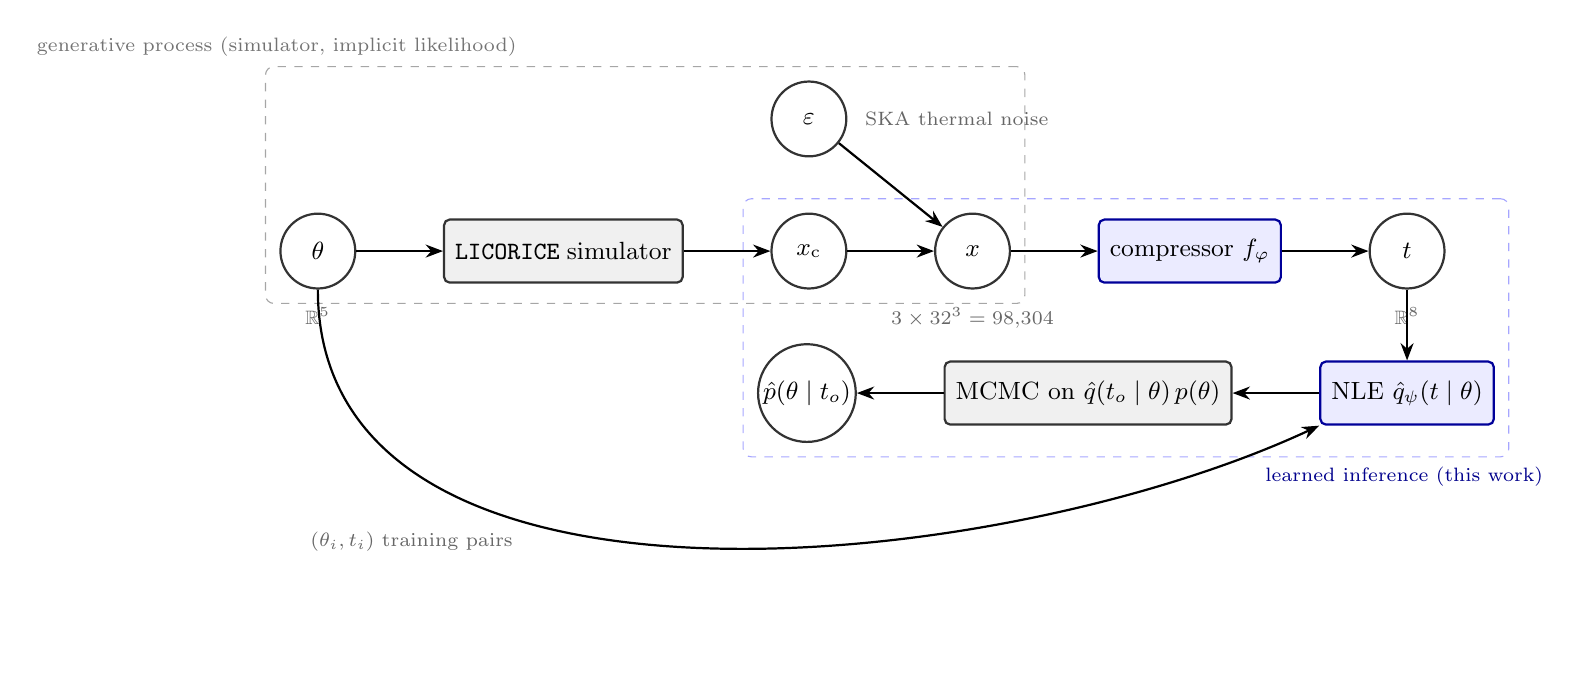
\begin{tikzpicture}[
  font=\small,
  node distance=9mm and 11mm,
  var/.style   ={circle, draw=black!80, thick, minimum size=9.5mm, inner sep=1pt},
  proc/.style  ={rectangle, rounded corners=2pt, draw=black!80, thick,
                 fill=black!6, minimum height=8mm, inner sep=4pt},
  learn/.style ={rectangle, rounded corners=2pt, draw=blue!60!black, thick,
                 fill=blue!8, minimum height=8mm, inner sep=4pt},
  dim/.style   ={font=\scriptsize, text=black!60},
  arr/.style   ={-{Stealth[length=2.2mm]}, thick},
]

% ---------------- generative process (top row) ----------------
\node[var] (theta) {$\theta$};
\node[dim, below=1mm of theta] {$\mathbb{R}^{5}$};

\node[proc, right=of theta] (sim) {\texttt{LICORICE}\;simulator};
\node[var, right=of sim] (xc) {$x_{\rm c}$};

\node[var, above=7mm of xc] (eps) {$\varepsilon$};
\node[dim, right=1mm of eps] {SKA thermal noise};

\node[var, right=of xc] (x) {$x$};
\node[dim, below=1mm of x] {$3\times32^3 = 98{,}304$};

\draw[arr] (theta) -- (sim);
\draw[arr] (sim) -- (xc);
\draw[arr] (xc) -- (x);
\draw[arr] (eps) -- (x);

% ---------------- inference pipeline (continues right / down) ----------------
\node[learn, right=of x] (f) {compressor $f_\varphi$};
\node[var, right=of f] (t) {$t$};
\node[dim, below=1mm of t] {$\mathbb{R}^{8}$};

\node[learn, below=of t] (nle) {NLE $\hat q_\psi(t\mid\theta)$};
\node[proc, left=of nle] (mcmc) {MCMC on $\hat q(t_o\mid\theta)\,p(\theta)$};
\node[var, left=of mcmc] (post) {$\hat p(\theta\mid t_o)$};

\draw[arr] (x) -- (f);
\draw[arr] (f) -- (t);
\draw[arr] (t) -- (nle);
\draw[arr] (theta.south) to[out=-90, in=-155, looseness=0.9]
  node[dim, pos=0.35, below left] {$(\theta_i, t_i)$ training pairs} (nle.south west);
\draw[arr] (nle) -- (mcmc);
\draw[arr] (mcmc) -- (post);

% ---------------- group boxes ----------------
\begin{scope}[on background layer]
  \node[fit=(theta)(sim)(eps)(x), draw=black!35, dashed, rounded corners=3pt,
        inner sep=5pt, label={[black!55]above left:{\scriptsize generative
        process (simulator, implicit likelihood)}}] {};
  \node[fit=(f)(t)(nle)(mcmc)(post), draw=blue!35, dashed, rounded corners=3pt,
        inner sep=5pt, label={[blue!55!black]below right:{\scriptsize learned
        inference (this work)}}] {};
\end{scope}

\end{tikzpicture}
\end{document}